\documentclass[12pt,english,dvipsnames,aspectratio=169,handout]{beamer}\usepackage[]{graphicx}\usepackage[]{xcolor}
% maxwidth is the original width if it is less than linewidth
% otherwise use linewidth (to make sure the graphics do not exceed the margin)
\makeatletter
\def\maxwidth{ %
  \ifdim\Gin@nat@width>\linewidth
    \linewidth
  \else
    \Gin@nat@width
  \fi
}
\makeatother

\definecolor{fgcolor}{rgb}{0.345, 0.345, 0.345}
\newcommand{\hlnum}[1]{\textcolor[rgb]{0.686,0.059,0.569}{#1}}%
\newcommand{\hlstr}[1]{\textcolor[rgb]{0.192,0.494,0.8}{#1}}%
\newcommand{\hlcom}[1]{\textcolor[rgb]{0.678,0.584,0.686}{\textit{#1}}}%
\newcommand{\hlopt}[1]{\textcolor[rgb]{0,0,0}{#1}}%
\newcommand{\hlstd}[1]{\textcolor[rgb]{0.345,0.345,0.345}{#1}}%
\newcommand{\hlkwa}[1]{\textcolor[rgb]{0.161,0.373,0.58}{\textbf{#1}}}%
\newcommand{\hlkwb}[1]{\textcolor[rgb]{0.69,0.353,0.396}{#1}}%
\newcommand{\hlkwc}[1]{\textcolor[rgb]{0.333,0.667,0.333}{#1}}%
\newcommand{\hlkwd}[1]{\textcolor[rgb]{0.737,0.353,0.396}{\textbf{#1}}}%
\let\hlipl\hlkwb

\usepackage{framed}
\makeatletter
\newenvironment{kframe}{%
 \def\at@end@of@kframe{}%
 \ifinner\ifhmode%
  \def\at@end@of@kframe{\end{minipage}}%
  \begin{minipage}{\columnwidth}%
 \fi\fi%
 \def\FrameCommand##1{\hskip\@totalleftmargin \hskip-\fboxsep
 \colorbox{shadecolor}{##1}\hskip-\fboxsep
     % There is no \\@totalrightmargin, so:
     \hskip-\linewidth \hskip-\@totalleftmargin \hskip\columnwidth}%
 \MakeFramed {\advance\hsize-\width
   \@totalleftmargin\z@ \linewidth\hsize
   \@setminipage}}%
 {\par\unskip\endMakeFramed%
 \at@end@of@kframe}
\makeatother

\definecolor{shadecolor}{rgb}{.97, .97, .97}
\definecolor{messagecolor}{rgb}{0, 0, 0}
\definecolor{warningcolor}{rgb}{1, 0, 1}
\definecolor{errorcolor}{rgb}{1, 0, 0}
\newenvironment{knitrout}{}{} % an empty environment to be redefined in TeX

\usepackage{alltt}
\usepackage{fontspec}
\setsansfont[Mapping=tex-text]{Fira Sans}
\setcounter{secnumdepth}{4}
\setcounter{tocdepth}{4}
\usepackage[normalem]{ulem}
\usepackage[T1]{fontenc}
\usepackage{dcolumn}
\usepackage{booktabs}
\usepackage{bm}
\usepackage{setspace}
\makeatletter
\usetheme{metropolis}
\setbeamertemplate{frame footer}{Bosancianu | Schaub | Hertie School}
\setbeamerfont{page number in head/foot}{size=\tiny}
\setbeamercolor{footline}{fg=gray}
\usepackage{xcolor}
\setbeamercovered{transparent}
\usepackage{tikz}
\usetikzlibrary{arrows, positioning,fit,shapes.misc}
\usepackage[labelformat=empty]{caption}
% For table captions in Beamer
\usepackage[sectionbib]{apacite}
\renewcommand{\bibliographytypesize}{\footnotesize}
\makeatletter
\let\st@rtbibsection\@bibnewpage
\let\st@rtbibchapter\@bibnewpage
\makeatother
\usepackage{amsmath, mathtools}
\usepackage{xunicode}
\usepackage{hyperref}
\graphicspath{{./figures/}} 
% Defines a checkmark
\def\checkmark{\tikz\fill[scale=0.4,color=orange](0,.35) -- (.25,0) -- (1,.7) -- (.25,.15) -- cycle;}
% Code for circles in Table cells
\newcounter{nodemarkers}
\newcommand\circletext[1]{%
    \tikz[overlay,remember picture] 
        \node (marker-\arabic{nodemarkers}-a) at (0,1.5ex) {};%
    #1%
    \tikz[overlay,remember picture]
        \node (marker-\arabic{nodemarkers}-b) at (0,0){};%
    \tikz[overlay,remember picture,inner sep=2pt]
        \node[draw,ellipse,fit=(marker-\arabic{nodemarkers}-a.center) (marker-\arabic{nodemarkers}-b.center)] {};%
    \stepcounter{nodemarkers}%
}
% wide itemize and enumerate
\newenvironment{wideitemize}{\itemize\addtolength{\itemsep}{.3em}}{\enditemize}
\newenvironment{wideenumerate}{\enumerate\addtolength{\itemsep}{.3em}}{\endenumerate}
% boxes
\def\boxitorange#1{%
  \smash{\color{orange}\fboxrule=1pt\relax\fboxsep=2pt\relax%
  \llap{\rlap{\fbox{\vphantom{0}\makebox[#1]{}}}~}}\ignorespaces
}
\def\boxitblue#1{%
  \smash{\color{blue}\fboxrule=1pt\relax\fboxsep=2pt\relax%
  \llap{\rlap{\fbox{\vphantom{0}\makebox[#1]{}}}~}}\ignorespaces
}
\newcommand{\indep}{\perp \!\!\!\! \perp}
\setbeamertemplate{itemize items}{\checkmark}
\usepackage{multirow}
\hypersetup{pdfauthor={Bosancianu and Schaub},
	pdftitle={Statistical Modeling and Causal Inference with R},
	pdfsubject={Week 8: DiD and Synthetic Controls},
	pdfkeywords={Berlin, Hertie, 2020, week 8}}
\title{\textsc{Statistical Modeling and Causal Inference with R}}
\subtitle{Week 8: DiD and Synthetic Controls}
\date{November 2, 2020}
\author{Manuel Bosancianu \hfill Max Schaub}
\institute{Hertie School of Governance}
\IfFileExists{upquote.sty}{\usepackage{upquote}}{}
\begin{document}
\maketitle

\begin{frame}
	\frametitle{Today's focus}
	\begin{itemize}
		\item A brief look at panel data
		\item Differences-in-difference / DiD
		\item Synthetic control method
	\end{itemize}
\end{frame}


\section{A brief look at panel data}

\begin{frame}
  \frametitle{A brief look at panel data}
\footnotesize

So far, we have not looked at observations over time. This will change in this and the next session, where we look at panel data, i.e.\ repeated observations from the same unit over time.

Notation: $Y_{it}$, $X_{it}$ etc. -- additional subscript $_t$ for time period, e.g. years 2014 and 2020

Representation 1: 

\scriptsize
\begin{table}\centering
\begin{tabular}{lccc}
\toprule
\multicolumn{4}{c}{Wide format table} \\
Unit c   & $Y_{c2014}$  & $Y_{c2020}$  & $D_c$  \\
\midrule
County A &  42.1     &    38.5   & 0         \\
County B &  41.2     &    40.2    & 1         \\
\ldots  &   \ldots  &  \ldots   & \ldots      \\
\bottomrule
\end{tabular}
\end{table}

One row for each unit $i$, different columns for different time periods $t$.

\end{frame}


\begin{frame}
  \frametitle{A brief look at panel data}
\footnotesize

Representation 2: 

\scriptsize
\begin{table}\centering
\begin{tabular}{lccc}
\toprule
\multicolumn{4}{c}{Long format table} \\
Unit c   & Year t  & $Y_c$  & $D_c$  \\
\midrule
County A & 2014  & 42.1 & 0   \\
County A & 2020  & 38.5 & 0   \\
County B & 2014  & 41.2 & 1   \\
County B & 2020  & 40.2 & 1   \\
\ldots  &\ldots &\ldots &\ldots  \\
\bottomrule
\end{tabular}
\end{table}

One row for each time period $t$, $t\times i$, one column for each outcome of covariate.

\end{frame}




\begin{frame}
  \frametitle{A brief look at panel data}
\footnotesize

Panel data interesting for causal inference
\begin{itemize}
  \item Allows for comparisons over time
  \item By looking at \emph{changes} of the same unit over time, we can
    \begin{itemize}\footnotesize
      \item Compare the same unit to itself, and by so doing\ldots
      \item control for all time-invariable characteristics of this unit.
      \item Compare \emph{changes} in outcomes between \emph{different} units 
    \end{itemize}
  \item More technical treatment of panel data during the next class
\end{itemize}

\end{frame}



\section{Difference-in-differences / DiD}

\begin{frame}
  \frametitle{DiD: General setting where DiD applies}
\footnotesize
A major use of panel data are difference-in-differences DiD Analyses. In the DiD approach, causal identification is established by comparing \textcolor{orange}{changes between treatment and control units over time}. DiD can potentially be used when:
\begin{enumerate}\footnotesize
  \item There is some event or measure that affects some units of a population but leaves others untouched.
\end{enumerate}
    \vspace{-3mm} \begin{itemize} \scriptsize
      \item A violent conflict starts in some regions but not others
      \item A schooling reform is introduced in some states but not others
      \item A tax reform affects certain projects but not other
      \item A diseases starts spreading in some areas but not others
      \item[] and many other settings\ldots
    \end{itemize} \vspace{-3mm}
\begin{enumerate} \footnotesize
  \item[2.] We have panel data from one or more points in time before the event happened/the measure was implemented, and after.
  \end{enumerate}
\end{frame}


\begin{frame}
  \frametitle{A motivating example: Effect of COVID-19 on electoral outcomes}
\footnotesize

Example: Effect of COVID-19 on municipal election in Bavaria on 15 March 2020 \cite{leininger_strategic_2020}

\begin{tabular}{ll}
Outcome:     & Vote share for the largest party (CSU) at the county level \\
`Treatment': &  COVID-19 cases (69/27 counties had cases) \\
Data:        & Electoral outcomes for 2014 and 2020, COVID-19 prevalence
\end{tabular}


\scriptsize
\begin{table}\centering
\begin{tabular}{lccc}
\toprule
\multicolumn{4}{c}{CSU vote shares } \\
Unit    & $Y_{2014}$  & $Y_{2020}$  & $D$  \\
\midrule
County A &  42.1     &    38.5   & 0         \\
County B &  41.2     &    40.2   & 1         \\
\ldots  &   \ldots  &  \ldots    & \ldots    \\
\bottomrule
\end{tabular}
\end{table}

\end{frame}



\begin{frame}
  \frametitle{Example: Possible counterfactuals}
\footnotesize

Given these data, what is the most convincing comparison?

A first approach would be to compare County A, which did not have a COVID-19 case with County B, which was affected by COVID-19, i.e.\ to use $Y_{c=A,t=2020}$ as counterfactual for $Y_{c=B,t=2020}$.

In our data: $41.2-42.2=-0.9$.

\scriptsize
\begin{table}\centering
\begin{tabular}{lccc}
\toprule
\multicolumn{4}{c}{CSU vote shares } \\
Unit    & $Y_{2014}$  & $Y_{2020}$  & $D$  \\
\midrule
County A &  \textcolor{orange}{42.1}     &    38.5   & 0         \\
County B &  \textcolor{orange}{41.2}     &    40.2   & 1         \\
\ldots  &   \ldots  &  \ldots   & \ldots   \\
\bottomrule
\end{tabular}
\end{table}
\end{frame}



\begin{frame}
  \frametitle{Example: possible counterfactuals}
\footnotesize

Such a comparison is obviously affected by a myriad of confounders, e.g.\ rural/urban, local economic development, education levels etc.

\scriptsize
Note: In practice, we would do this for all 96 counties, and would use regression and matching methods to try to make the treatment assignment as independent as possible from such confounding factors. 

With two-period data, we can use the electoral outcome during the previous election as a powerful control variable that captures many of the idiosyncracies that make counties different in potential outcomes.  

\vspace{1cm}
\end{frame}




\begin{frame}
  \frametitle{Example: Possible counterfactuals}
\footnotesize

Another simple comparison would be to look a the affected County B before and after it was affected by COVID-19, i.e.\ to use $Y_{c=B,t=2014}$ as counterfactual for $Y_{c=B,t=2020}$

In our data: $40.2-41.2=-1$.

\scriptsize
\begin{table}\centering
\begin{tabular}{lccc}
\toprule
\multicolumn{4}{c}{CSU vote shares } \\
Unit    & $Y_{2014}$  & $Y_{2020}$  & $D$  \\
\midrule
County A &  42.1     &    38.5   & 0         \\
County B &  \textcolor{orange}{41.2}     &    \textcolor{orange}{40.2}    & 1       \\
\ldots  &   \ldots  &  \ldots   & \ldots    \\
\bottomrule
\end{tabular}
\end{table}

\end{frame}



\begin{frame}
  \frametitle{Example: Possible counterfactuals}
\footnotesize

This addresses the concern with time-fixed confounders such as whether the county is more urban or rural, and also largely addresses slow-moving factors such as age structure, average level of education etc.

However, again there are many other factors that may have influenced electoral outcomes over time, e.g.\ the appearance of a new party (the AfD), a change in environmental consciousness, a change from a less popular to a more popular leader, etc.

Any of these could be at the root of the effect we are observing.

\vspace{1cm}
  
\end{frame}




\begin{frame}
  \frametitle{Example: Possible counterfactuals, DiD}
\footnotesize

The idea of the differences-in-differences approach is to address the problems of between-unit and over-time comparison by \textcolor{orange}{comparing over-time differences between units}, i.e. we use $Y_{c=A,t=2020} - Y_{c=A,t=2014}$ as a counterfactual for  $Y_{c=B,t=2020} - Y_{c=B,t=2014}$.

\scriptsize
\begin{table}\centering
\begin{tabular}{lcccc}
\toprule
\multicolumn{5}{c}{CSU vote shares } \\
Unit    & $Y_{2014}$  & $Y_{2020}$  & $D$ & $\Delta Y_{2020-2014}$  \\
\midrule
County A &  42.1     &    38.5   & 0  &   -3.6     \\
County B &  41.2     &    40.2   & 1  &     -1  \\
\midrule \midrule
$\Delta$     &  -0.9     &     1.7   &    & \textcolor{orange}{2.6} \\
\bottomrule
\end{tabular}
\end{table}

\footnotesize
In our data: $(40.2-41.2)-(38.5-42.1)=2.6$.
\end{frame}


\begin{frame}
  \frametitle{DiD: Basic idea}
\footnotesize

The DiD estimator captures confounders that do not vary over time because it compares units to itself.

It also has the potential to capture confounders time-varying confounders that are the same for all units whether treatment or control. 

The specific identifying assumption is that in the absence of the treatment (COVID-19), the outcome would have followed a time-invariant unit (here: county) effect and a time effect that is common across all counties, i.e.\

$E[Y_{0ct}|D,t] = \gamma_c + \lambda_t$

\end{frame}


\begin{frame}
  \frametitle{DiD: Counterfactual}
\footnotesize

Graphical representation of treatment effect given the counterfactual:

	 \begin{figure} 
    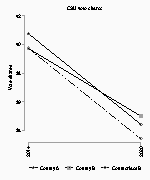
\includegraphics[height=.7\textheight,keepaspectratio=true]{../04-figures/08/01-twoperiod.pdf}
    \end{figure}

\end{frame}



\begin{frame}
  \frametitle{DiD: Assumption}
\footnotesize

For the identifying assumption to hold, the \textcolor{orange}{parallel trends assumption} has to be met: the claim that in the absence of treatment, treatment and control group outcomes would have moved in parallel.

This assumption in itself is not testable since we cannot observe the potential outcome $Y_{0ct+1}|D_c=1$.

However, the parallel trends assumption implies that prior to the treatment, the units in the treatment condition should have followed the same trend -- they should have moved in a similar way in response to external influences. 

\end{frame}


\begin{frame}
  \frametitle{DiD: Parallel trends}
\footnotesize

Graphical representation of common trends prior to treatment:
	 \begin{figure} 
    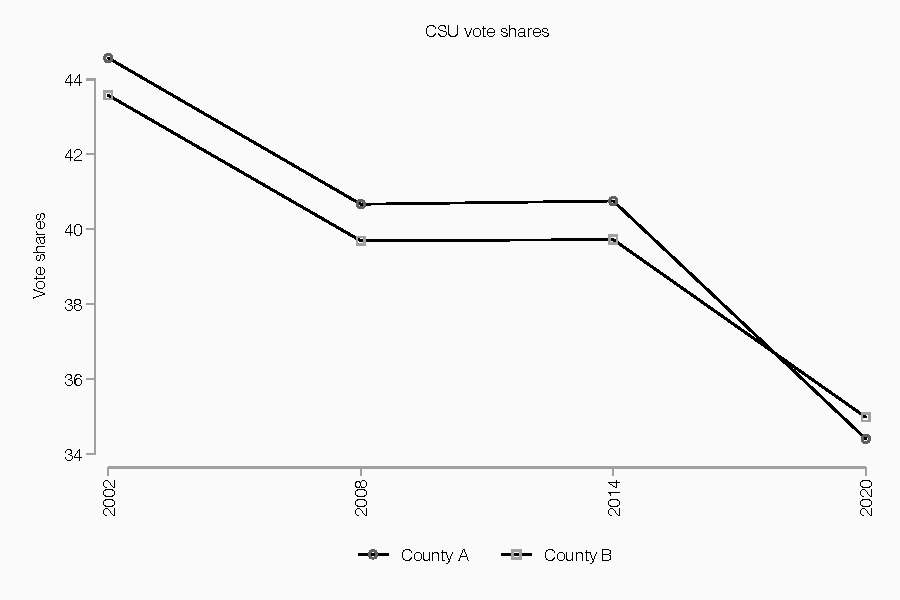
\includegraphics[height=.7\textheight,keepaspectratio=true]{../04-figures/08/02-fourperiod.pdf}
    \end{figure}
\end{frame}


\begin{frame}
  \frametitle{DiD: Calculation}
\footnotesize

Usually, we consider more than two units. For example, in the election dataset there are 96 counties.

\scriptsize
\begin{table}\centering
\begin{tabular}{lccc}
\toprule
\multicolumn{4}{c}{CSU vote shares } \\
Unit    & $Y_{2014}$  & $Y_{2020}$  & $D$  \\
\midrule
County A &  42.1     &    38.5   & 0         \\
County B &  41.2     &    40.2   & 1         \\
County C &  47.4     &    36.4   & 0         \\
County D &  49.0     &    40.2   & 0         \\
County E &  38.2     &    34.3   & 1         \\
County F &  43.9     &    39.1   & 1         \\
\ldots  &   \ldots  &  \ldots    & \ldots    \\
\bottomrule
\end{tabular}
\end{table}

\end{frame}


\begin{frame}
  \frametitle{DiD: Calculation}
\footnotesize

In such cases, we use group averages to calculate the DiD, i.e.\

\begin{align*}
DiD &= \{E[Y_{1c}|D=1,t=2020] - E[Y_{0c}|D=0,t=2020]\} - \\ 
    &  \{E[Y_{1c}|D=1,t=2014] - E[Y_{0c}|D=0,t=2014]\}
\end{align*}

There are several ways to calculate the DiD:
  \begin{enumerate}
    \item Manually, by calculating averages for subgroups defined by $D$ and $t$
    \item Regressing first differences on the treatment indicator (in `wide' data format)
    \item Using the regression formulation of the DiD model (in `long' data format)
  \end{enumerate}

\vspace{1cm}
\end{frame}



\begin{frame}
  \frametitle{DiD: Calculation}
\footnotesize

1. `Manually

\begin{align*}
DiD &= \{E[Y_{1c}|D=1,t=2020] - E[Y_{0c}|D=0,t=2020]\} - \\ 
    &  \{E[Y_{1c}|D=1,t=2014] - E[Y_{0c}|D=0,t=2014]\} \\
    &= (34.99-34.41) - \\
    &   (39.73-40.76) \\
    &= 1.61
\end{align*}

\vspace{1cm}
\end{frame}


\begin{frame}
  \frametitle{DiD: Calculation}
\footnotesize

2. Regression of first differences on treatment indicator (in `wide' data format) using $\Delta Y_{c_{2014-2020}} = \alpha + \delta D_c + \Delta u_c$ 
\vspace{5mm}

\scriptsize
\centering
\begin{tabular}{l*{1}{c}}
\toprule
          &\multicolumn{1}{c}{$CSU_{2014-2020}$}\\
\midrule
Treat &     1.61\textsuperscript{**} \\
          &   (0.79)         \\
Intercept   &    -6.34\textsuperscript{***}\\
          &   (0.71)         \\
\midrule
\(N\)     &       96         \\
\(R^{2}\) &     0.05         \\
\bottomrule
\multicolumn{2}{l}{ Standard errors in parentheses}\\
\multicolumn{2}{l}{ \textsuperscript{*} \(p<0.10\), \textsuperscript{**} \(p<0.05\), \textsuperscript{***} \(p<0.01\)}\\
\end{tabular}
\end{frame}




\begin{frame}
  \frametitle{DiD: Calculation}
\footnotesize

3. Using the regression formulation of the DiD model, by far the most common way to calculate the DiD for the two-period, two-conditions case, i.e.\ : $DiD = Y_{ct} = \alpha + \beta D_c + \gamma Post_t + \delta (D_c\times Post_t) + u_{ct}$ \scriptsize with $Post_t$ standing for the post-treatment period, i.e.\ the year 2020 \footnotesize

The coefficients estimated by the regression model translate into the observed outcomes as follows:

\scriptsize
\begin{table}\centering
\begin{tabular}{lcc}
\toprule
            &   $t=2014$ (pre)      & $t=2020$ (post) \\
\midrule
$D_c=0$     & $E[Y_{0c2014}|D_c=0]$           & $E[Y_{0c2020}|D_c=0]$ \\
$D_c=1$    & $E[Y_{1c2014}|D_c=1]$            & $E[Y_{1c2020}|D_c=1]$ \\
\midrule
$D_c=0$     & $\alpha$           & $\alpha + \gamma$ \\
$D_c=1$    & $\alpha + \beta$   & $\alpha + \beta + \gamma + \delta$ \\
\bottomrule
\end{tabular}
\end{table}

\end{frame}



\begin{frame}
  \frametitle{DiD: Regression estimators}
\footnotesize

Regression results from our example data:

\scriptsize
\centering
\begin{tabular}{l*{1}{c}}
\toprule
          &\multicolumn{1}{c}{Share CSU}\\
\midrule
Treat     &    -1.03         \\
          &   (1.56)         \\
Post      &    -6.34\textsuperscript{***}\\
          &   (0.72)         \\
$Treat\times Post$&     1.61\textsuperscript{**} \\
          &   (0.79)         \\
Intercept    &    40.76\textsuperscript{***}\\
          &   (1.39)         \\
\midrule
\(N\)     &      192         \\
\(R^{2}\) &     0.16         \\
\bottomrule
\multicolumn{2}{l}{Standard errors in parentheses}\\
\multicolumn{2}{l}{ \textsuperscript{*} \(p<0.10\), \textsuperscript{**} \(p<0.05\), \textsuperscript{***} \(p<0.01\)}\\
\end{tabular}
\end{frame}




\begin{frame}
  \frametitle{DiD: Regression estimators}
\footnotesize

We can use these results and the insights into the interpretation of the coefficients to recover the `manual' DiD estimator:

\scriptsize
\begin{table}\centering
\begin{tabular}{lcc}
\toprule
            &   $t=2014$ (pre)      & $t=2020$ (post) \\
\midrule
$D_c=0$      & $40.76$            & $40.76 + (-6.34) = 34.42$ \\
$D_c=1$    & $40.76 + (-1.03) =39.73 $ & $40.76 + (-1.03) + (-6.34) + 1.61 = 35.00$ \\
\bottomrule
\end{tabular}
\end{table}

\footnotesize
which gives: $DiD = (35.00-39.73) - (34.42-40.76) = 1.61$

Easier to just look at $\delta$, of course\ldots

\end{frame}




\begin{frame}
  \frametitle{DiD: Generalized DiD regression estimator}
\footnotesize

The DiD model can also be expressed as a two-way fixed effects model in the so-called generalized DiD:

$DiD = Y_{ct} = \lambda_c + \gamma_t + \delta D_{ct} + u_{ct}$

where $\lambda_c$ are dummies for the units, $\gamma_t$ for the included time periods, and $D_{ct}$ indicates whether a unit $c$ is in its treated or untreated state at a given point in time $t$. 

This model also compares within-unit deviations in outcomes between units at the same time, but accommodates situations where some units have their treatment `switched on' at different points in time.

\end{frame}



\begin{frame}
  \frametitle{DiD: Regression estimators}
\footnotesize

The regression formulation of the DiD has the advantage that we can add additional control variables, notably factors varying at the level of the unit over time. E.g.\

$DiD = Y_{ct} = \lambda_c + \gamma_t + \delta D_{ct} + \bm{\rho X_{ct}} + u_{ct}$

Such factors $\rho X_{ct}$ could be the economic development at the county level between 2014 and 2020, population dynamics, refugee settlement, etc.

Including such predictors should increase the precision of our estimates.

The framework also allows for non-dichotomous treatments/a treatment of varying intensity e.g.\ the number of COVID-19 cases.

\end{frame}

\begin{frame}
  \frametitle{DiD: Regression estimators}
\footnotesize
DiD including controls: outcome is \% CSU vote share.

\tiny
\centering
\begin{tabular}{l*{1}{c}}
\toprule
Treat &    -2.17         \\
          &   (1.56)         \\
Post      &    -7.07\textsuperscript{***}\\
          &   (1.05)         \\
$Treat\times Post$ &     1.62\textsuperscript{**} \\
          &   (0.80)         \\
Diff popdens&    -0.03\textsuperscript{*}  \\
          &   (0.02)         \\
Diff foreign&    -0.03         \\
          &   (0.20)         \\
Diff unemployrate &    -0.12         \\
          &   (0.08)         \\
Diff age 60 and over &     0.40         \\
          &   (0.31)         \\
Diff employees&     0.06         \\
          &   (0.06)         \\
Intercept   &    36.29\textsuperscript{***}\\
          &   (7.60)         \\
\midrule
\(N\)     &      192         \\
\(R^{2}\) &     0.34         \\
\bottomrule
\multicolumn{2}{l}{Standard errors in parentheses}\\
\multicolumn{2}{l}{ \textsuperscript{*} \(p<0.10\), \textsuperscript{**} \(p<0.05\), \textsuperscript{***} \(p<0.01\)}\\
\end{tabular}
\end{frame}




\begin{frame}
  \frametitle{DiD: Leads in regression estimators}
\footnotesize

The generalized formulation of the DiD framework also allows us to test the common trends assumption by including \textcolor{orange}{`leads'} -- `treatment effects' for the periods leading up to the actual treatment.

Practically this is done by including the interactions between the treatment indicator and year dummies, but leaving out the pre-treatment period (the year 2014 in our example) as reference period:

$Y_{ct} = \lambda_c + \gamma_t + \delta_{t-3} D_{c_{2002}} + \delta_{t-2} D_{c_{2008}} + \delta_t D_{c_{2020}} + \rho X_{ct} + u_{ct}$

If the common trends assumption holds, the coefficients for $\delta_{t-3}$ and $\delta_{t-2}$ should be small and statistically insignificant.

Another way of thinking about `leads' is in terms of \textcolor{orange}{placebo treatments}: you are `assuming' that the treatment took place in 2002 or 2008 -- and show that this imagined treatment has no effect!

\end{frame}


\begin{frame}
  \frametitle{DiD: Leads in regression estimators}
\footnotesize

Recall the graphical representation of the common trends prior to treatment:
	 \begin{figure} 
    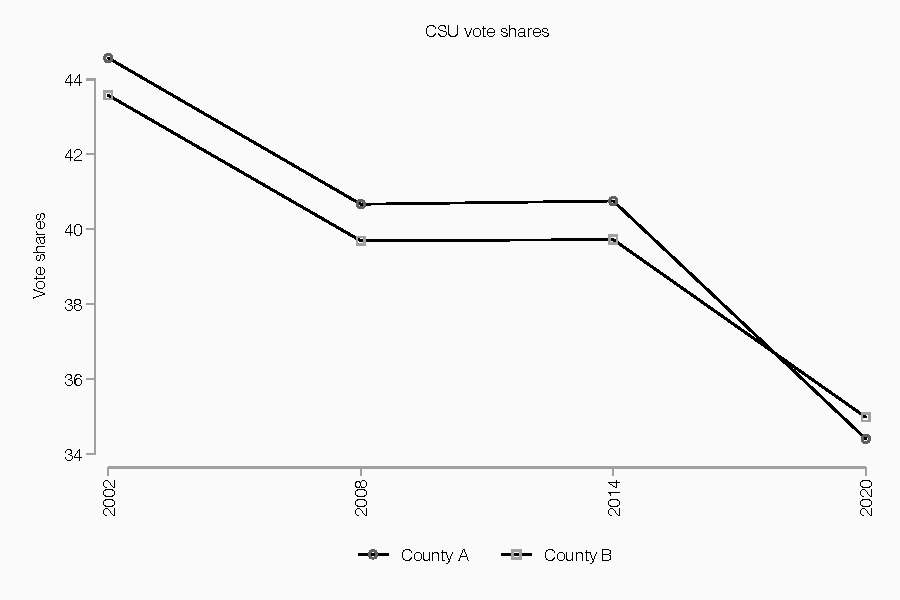
\includegraphics[height=.6\textheight,keepaspectratio=true]{../04-figures/08/02-fourperiod.pdf}
    \end{figure}
\end{frame}



\begin{frame}
  \frametitle{Two-period diff-in-diff}
\footnotesize

Plot of `leads' in DiD framework:

	 \begin{figure} 
    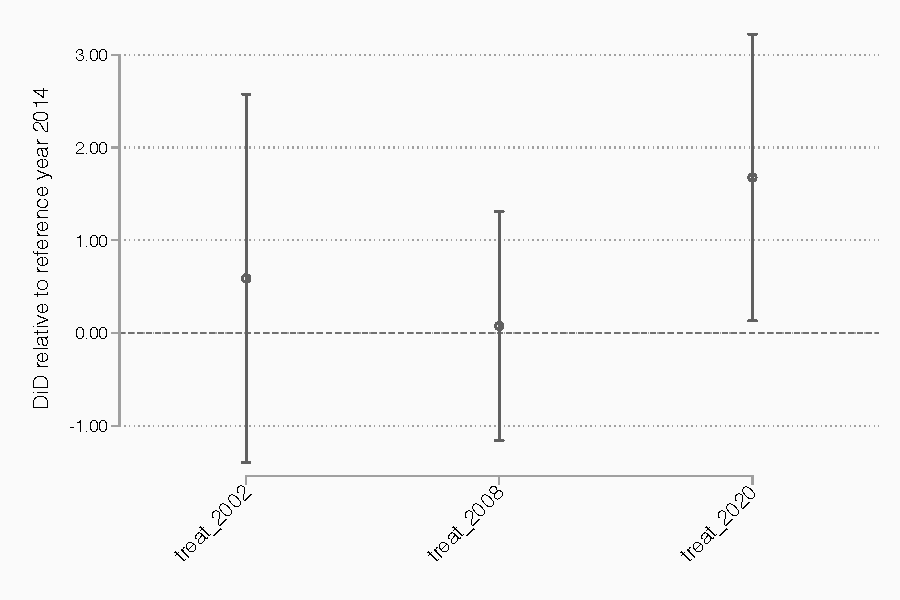
\includegraphics[height=.55\textheight,keepaspectratio=true]{../04-figures/08/03-lead.pdf}
    \end{figure}
\vspace{-5mm}    
Plotted `leads' are the DiD between 2002 and 2014, 2008 and 2014, and the third coefficient is the difference-in-differences between 2020 and 2014, respectively.

\end{frame}



\begin{frame}
  \frametitle{DiD: Lags in regression estimators}
\footnotesize

In the same way, we can include `lag' -- `treatment effects' for the periods after the actual treatment occurred (cp. Autor \citeyear{autor_outsourcing_2003} for the classic reference using both `leads' and `lags').

These can help to see how long-lasting the effect is. Again, this is done by adding interactions between the treatment indicator and year dummies. 

The full model may then look like this (here based on an example from Hakelberg and Schaub \citeyear{hakelberg_redistributive_2018}): 

\begin{equation*}
Y_{ct} = \lambda_c + \gamma_t + \sum_{t=2005}^{2009} \delta_t D_{ct} + \sum_{t=2011}^{2015} \delta_t D_{ct} + \rho X_{ct} + u_{ct}
\end{equation*}

\end{frame}


\begin{frame}
  \frametitle{DiD: Lags in regression estimators}
\footnotesize

Example studying the effect of the FATCA (Foreign Account Tax Compliance Act) reform in the U.S.\ in 2011 on tax havens \cite{hakelberg_redistributive_2018}. 

	 \begin{figure} 
    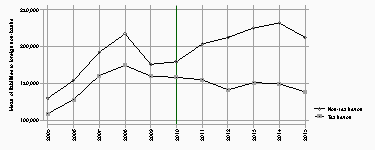
\includegraphics[height=.65\textheight,keepaspectratio=true]{../04-figures/08/04-fatcatrend.pdf}
    \end{figure}

\end{frame}


\begin{frame}
  \frametitle{DiD: Lags in regression estimators}
\footnotesize

Graphical representation of inclusion of `lags' in DiD framework from Hakelberg and Schaub \citeyear{hakelberg_redistributive_2018}.

	 \begin{figure} 
    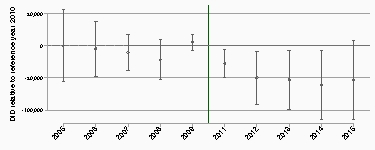
\includegraphics[height=.5\textheight,keepaspectratio=true]{../04-figures/08/05-fatca.pdf}
    \end{figure}

The plot shows that the `placebo treatments' between 2005 and 2009 -- imagined reforms prior to the actual reform in 2011 -- had no effect on liabilities, whereas the real reform in 2011 had a clear, additive effect every single year 2011-2014.

\end{frame}



\begin{frame}
  \frametitle{DiD: Further issues}
\footnotesize

When using DiD, standard errors need to be adjusted. This is because observations from the same unit for two or more time periods are likelily to be \textcolor{orange}{serially correlated}, i.e.\ not independent from each other. 

For example, the vote share 2014 is correlated with the vote share 2020. The adjustment can be done by using \emph{clustered standard errors} or \emph{bootstrapping} (estimating the standard errors by sampling sub-samples from the data that give an estimate of the variability of the estimated DiD effect).

The DiD framework is useful for the analysis of almost any panel data set where the treatment and control group follow a common trend pre-treatment.

However, even though the common trends assumption can be relaxed by allowing for units to follow their own time trends (cp.\ Angrist and Pischke \citeyear{angrist_mostly_2009}), most scholars would agree that DiD conceptually makes most sense when there are parallel trends. 

So what if there are no parallel trends?

\end{frame}



\section{Synthetic control method}

\begin{frame}
  \frametitle{Synthetic control method: General setting}
\footnotesize
The synthetic control method serves to estimate the causal effect of an intervention or treatment by comparing a treated unit over time to a synthetic control unit that is constructed as a weighted average of potential control or `donor' units.

\vspace{3cm}
\end{frame}


\begin{frame}
  \frametitle{Synthetic control method: General setting}
\footnotesize

The synthetic control method might be used in cases:
\begin{enumerate}
  \item Where there is no optimal control/a lack of a common trend
  \item Where the treatment unit is $n=1$ -- inspired by qualitative \textcolor{orange}{comparative case studies} \vspace{-3mm}
\end{enumerate}
    \begin{itemize} \scriptsize
      \item Violent conflict: terrorism in the Basque country \cite{abadie_economic_2003}
      \item Legal changes in a single state: tobacco law in California \cite{abadie_synthetic_2010}
      \item Rare historical events: German reunification \cite{abadie_comparative_2015}
    \end{itemize} \vspace{-3mm}
\begin{enumerate} \footnotesize
  \item[3.] We have panel data from several points in time before the event happened/the measure was implemented, and after 
  \end{enumerate}
\end{frame}




\begin{frame}
  \frametitle{Synthetic control method: Comparison with DiD}
\footnotesize
Similar idea to DiD: 
\begin{itemize} 
  \item Estimate treatment effect by comparing the trends in outcomes in a treatment unit to that of control unit
\end{itemize}
Differences:
\begin{itemize} 
  \item Explicitly restricted to a single treatment unit, and a single, composite control unit
  \item Rather than relying on actually observed cases, constructs optimal control unit from pool of control units
  \item The synthetic control is contructed as a weighted average of the units in the donor pool 
  \item Different (less formal) statistical tests to gage plausibility of estimated effect
\end{itemize} 
\end{frame}



\begin{frame}
  \frametitle{Synthetic control method: Example}
\footnotesize

What is the effect of an anti-smoking measure in California (Proposition 99, enacted in 1989) on cigarette sales \cite{abadie_synthetic_2010}?

Idea: compare development in cigarette sales in California to similar state.

Problems:
\begin{itemize} 
  \item No other unit(s) with similar pre-Proposition trajectory of cigarette sales
  \item Single treated case (California) -- how to do statistical inference/test uniqueness of effect?
\end{itemize} 

\vspace{1cm}

\end{frame}


\begin{frame}
  \frametitle{Example: Lack of control group}
\footnotesize

Figure demonstrating that California cigarette sales followed different trajectory from rest of the U.S.\

	 \begin{figure} 
    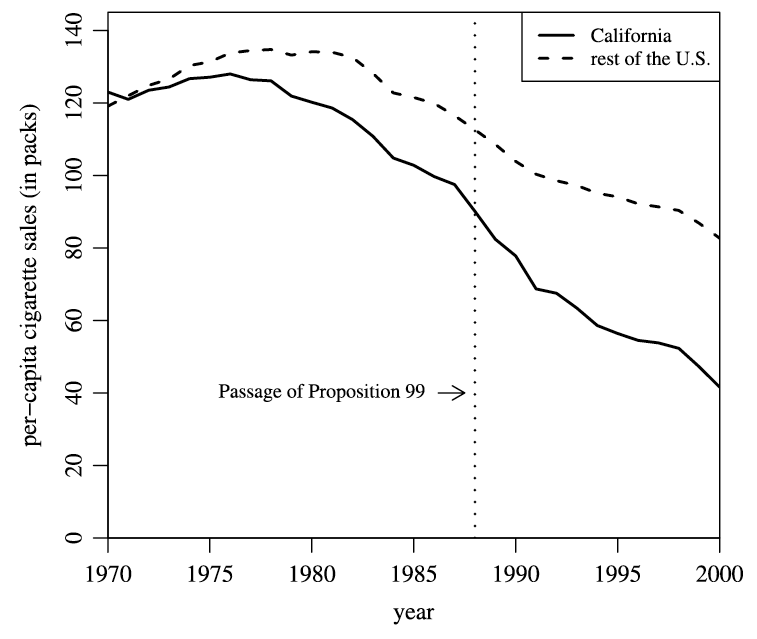
\includegraphics[height=.65\textheight,keepaspectratio=true]{../04-figures/08/06-abadie1}
    \end{figure}

\end{frame}




\begin{frame}
  \frametitle{Synthetic control group: Distance measure}
\footnotesize

Abadie, Diamond, and Hainmueller \citeyear{abadie_synthetic_2010} (following Abadie and Gardeazabal 2003) address this problem by constructing a `synthetic' California out of a weighted sample of 38 other U.S.\ states.

Technically, the idea is as follows:

Assume that $X_1$ is a vector holding covariate values from the treatment unit (California), and $X_0$ is a matrix holding values for the same covariates for all the control units (the 38 other states), we can find a vector $W^*$ with weights for each control unit that minimize the distance between the treatment case and the control units.

\vspace{10mm}

\end{frame}




\begin{frame}
  \frametitle{Synthetic control group: Distance measure}
\footnotesize

Specifically, Abadie, Diamond, and Hainmueller \citeyear{abadie_synthetic_2010} look for a vector $W^*$ that minimizes

\begin{equation*} 
\sum_{m=1}^{k} v_m(X_{1m}-X_{0m}W)^2
\end{equation*}

i.e.\ the squared distance between all the values $m$ of the vector $X_1$ minus the value for the same covariate $m$ in the vector of the control units $X_0$ times a weight $v_m$ that captures the importance of this covariate for predicting the outcome of interest. 

The weight $v_m$ is found with methods from machine learning.

\end{frame}



\begin{frame}
  \frametitle{Example: Selected weights}
\footnotesize

Table showing the weights assigned to the units of the door pool to create the `synthetic California'

	 \begin{figure} 
    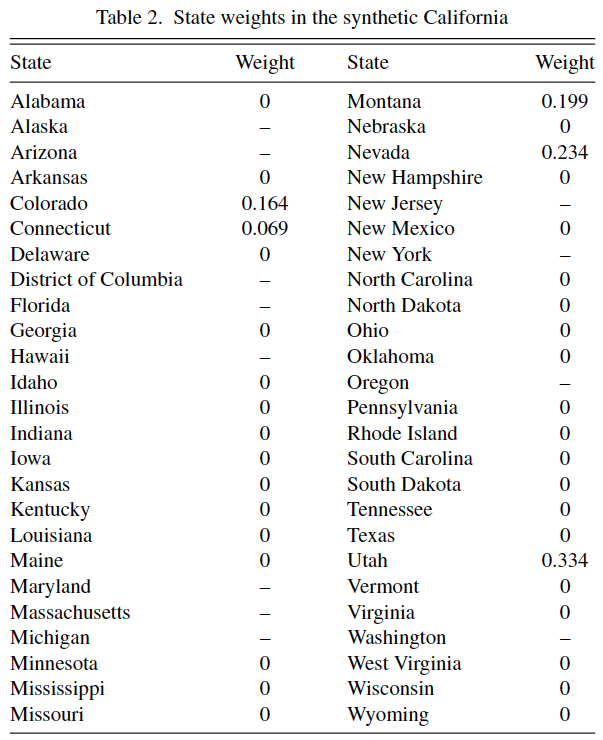
\includegraphics[height=.65\textheight,keepaspectratio=true]{../04-figures/08/07-abadietable2}
    \end{figure}
 
\end{frame}




\begin{frame}
  \frametitle{Example: Synthetic California}
\footnotesize

The `synthetic California' closely tracks cigarette sales in the real California until the Proposition 99 is introduced, from where on the treated case and the synthetic control diverge.

	 \begin{figure} 
    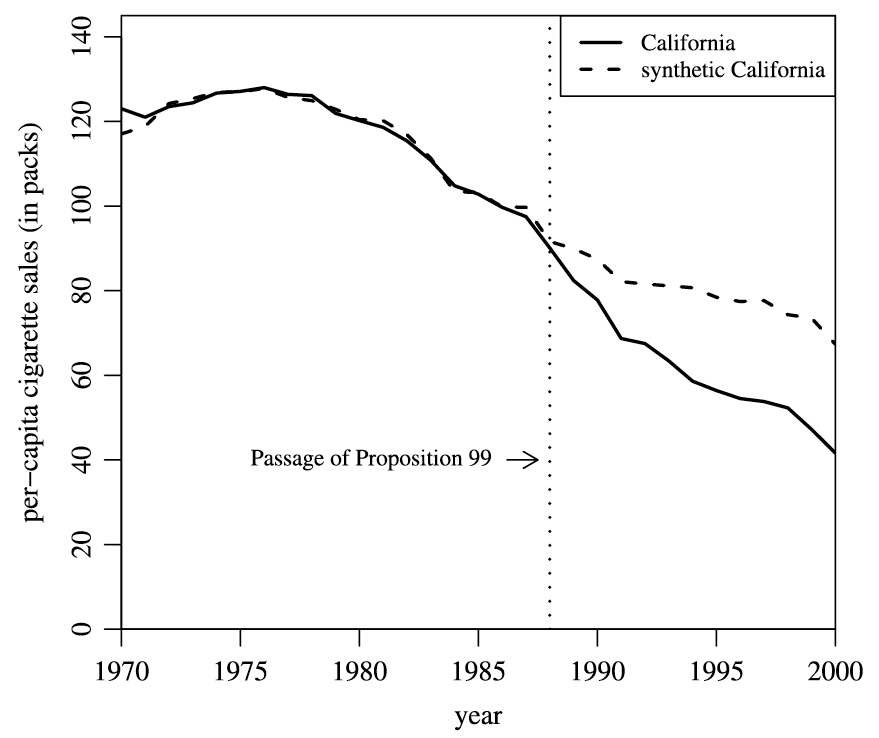
\includegraphics[height=.5\textheight,keepaspectratio=true]{../04-figures/08/08-abadie2}
    \end{figure}

From this they conclude that the treatment \emph{caused} cigarette sales to decline. 
\end{frame}



\begin{frame}
  \frametitle{Synthetic control group: Estimator}
\footnotesize

The treatment effect is given by the comparison of postintervention outcomes (cigarette sales post Proposition 99) between the treated unit and the synthetic control, i.e.\ $Y_1 − Y_0W^∗$, which is calculated for each post-treatment period $t$ as:

\begin{equation*} 
Y_{1t}-\sum_{j=2}^{J+1} \omega^*_jY_{jt}
\end{equation*}

i.e.\ the difference between the outcome for the treated unit ($j=1$) minus the sum of the weighted outcomes of the control unit (indexed $j=2$, $j=3$, etc.).

\vspace{10mm}

\end{frame}



\begin{frame}
  \frametitle{Synthetic control method: Inference}
\footnotesize

The problem is that with such an approach is that we are left with a 1:1 comparison, meaning that usual statistical tests (which are based on comparing the \emph{distributions} betweent the treatment and the control group) do not apply.

Instead of the usual `frequentist' tests, the authors conduct a series of other tests, including ``in-time placebos'' (pretending the treatment took place in another year, just as is done with the inclusion of `leads' in DiD), and ``in-space placebos.'' 

\vspace{10mm}
\end{frame}


\begin{frame}
  \frametitle{Synthetic control method: Inference}
\footnotesize

The idea of the ``in-space placebo'' tests is to

\begin{enumerate}
  \item estimate hypothetical treatment effects for every potential control unit in the donor pool
  \item rank treatment effects and determine which share of hypothetical treatments produce a stronger treatment effect than the one observed in the studied case
  \item which then this gives us a p-value; for example, if 92\% of observations produce a smaller treatment effect, the associated p-value of the treatment effect in focus (that for California) is $p=0.08$
\end{enumerate} 
\end{frame}



\begin{frame}
  \frametitle{Example: Inference}
\footnotesize

Graphical representation of "in-space placebo:"

	 \begin{figure} 
    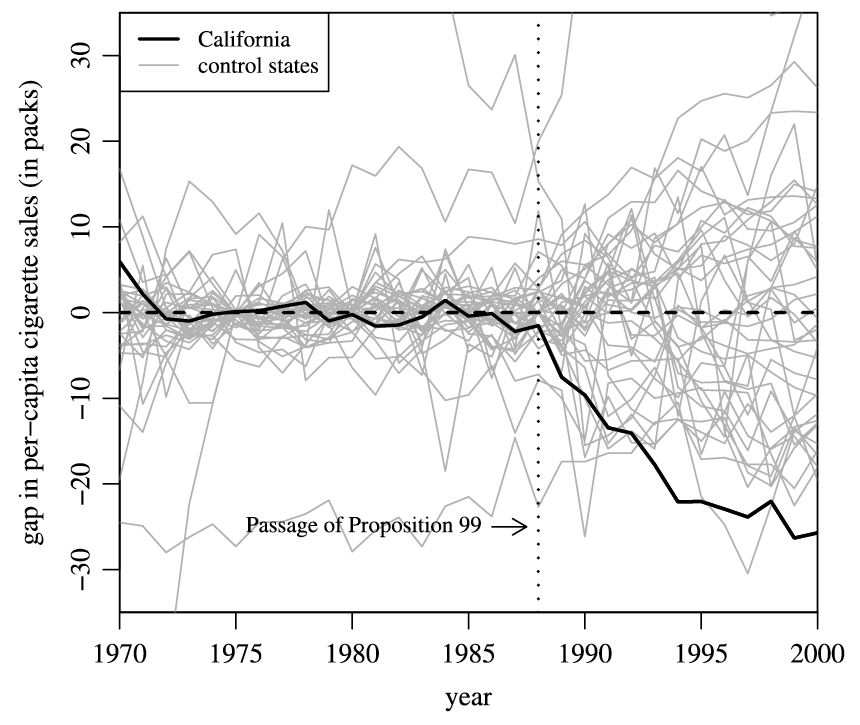
\includegraphics[height=.55\textheight,keepaspectratio=true]{../04-figures/08/09-abadie3}
    \end{figure}
\scriptsize
The different paths show differences in cigarette sales between each control unit and it's best fitting synthetic control over time. The treatment effect for California clearly stands out as one of the strongest effects, lending credibility to the claim that the reform here had a causal impact.
\end{frame}


% END
\begin{frame}
\begin{center}
    \LARGE Thank you for watching, and see you next Monday!
\end{center}
\end{frame}

% REFERENCES %

\begin{frame}[allowframebreaks]
\frametitle{References}
\bibliographystyle{apacite}
\scriptsize\bibliography{../Bibliography}
\end{frame}

\end{document}
